\documentclass[11pt,a4paper]{article}

\usepackage[T1]{fontenc}
\usepackage[utf8]{inputenc}
\usepackage{lmodern}
\usepackage[margin=2.5cm]{geometry}
\usepackage{amsmath,amssymb}
\usepackage{booktabs}
\usepackage{graphicx}
\usepackage{xcolor}
\usepackage{tikz}
\usetikzlibrary{positioning,arrows.meta}
\usepackage[numbers,sort&compress]{natbib}
\usepackage[colorlinks=true,linkcolor=blue!50!black,citecolor=blue!50!black,urlcolor=blue!50!black]{hyperref}
\usepackage{enumitem}
\setlist{nosep,leftmargin=*}

\title{Can a Small Model Switch Tokenizers?\\[4pt]
\large Reproducing ``Getting the most out of your tokenizer for pre-training and domain adaptation'' at small scale, then making the switch cheaper for code and Chinese\\[6pt]
\normalsize Final Project Proposal}
\author{[Member names] \\ {[Group name]} \quad $\cdot$ \quad [Course name]}
\date{October 27, 2026}

\begin{document}
\maketitle

\begin{abstract}
Tokenizers are rarely re-tuned when a pre-trained language model is adapted to a new domain, although a domain-specific tokenizer can encode the same text with far fewer tokens. \citet{dagan2024tokenizer} show that the tokenizer of a 1.5B or 7B code model can be replaced without loss in accuracy, but only after around 50B tokens of fine-tuning. Our project has three phases. \textbf{Phase~1} reproduces their tokenizer-design study and tokenizer swap on code, at the scale of a student project: GPT-2 small (124M parameters) and budgets of 50M and 200M tokens on consumer GPUs. \textbf{Phase~2} introduces a \emph{progressive tokenizer transition}, in which training sequences are encoded with the new tokenizer with a probability that increases from 0 to 1, and compares it with the paper's abrupt swap on code, a domain close to English, and on Chinese, a domain far from it. \textbf{Phase~3} (optional) tests whether a model trained this way tolerates shorter, non-standard encodings at inference.
\end{abstract}

%=====================================================================
\section{Motivation}
\label{sec:motivation}

Tokenization is one of the first decisions taken in a language-modeling project and one of the least revisited. When a general-purpose model is specialized, its tokenizer is usually inherited unchanged: Code Llama~\citep{roziere2023codellama} reuses the tokenizer of Llama~\citep{touvron2023llama}, which was trained mostly on natural language. Yet tokenizers trained on the target domain compress it far better. The InCoder tokenizer~\citep{fried2023incoder} needs about 26\% fewer tokens than Llama's to encode the same source code~\citep[Table~1]{dagan2024tokenizer}. The gap is even larger for languages far from English: the GPT-2 tokenizer~\citep{radford2019gpt2} encodes 4.44 bytes of English per token but only 2.19 bytes of multilingual text~\citep[Table~11]{dagan2024tokenizer}, and every Chinese character takes three bytes in UTF-8.

Compression matters because, in a decoder-only Transformer, each token costs one forward pass. Fewer tokens means faster and cheaper generation, a longer effective context, and more text seen per unit of training compute.

A better tokenizer therefore pays off at inference, but switching to it is expensive. In the experiments of \citet{dagan2024tokenizer}, a model whose tokenizer was replaced needed around 50B tokens of fine-tuning to match the original. Such budgets are out of reach for students and small labs. We ask two questions: \emph{does the paper's recipe still work at small scale}, and \emph{can we make the switch cheaper}?

%=====================================================================
\section{Related Works}
\label{sec:related}

\paragraph{Base paper.} \citet{dagan2024tokenizer} study tokenization for code LLMs and identify three levers that control how well a BPE tokenizer~\citep{sennrich2016bpe} compresses a target domain:
\begin{enumerate}
  \item \textbf{Training data.} Training the tokenizer on the target data mix (they use 70\% code, 30\% English) improves in-domain compression.
  \item \textbf{Pre-tokenization.} The regular expression applied before BPE decides which character sequences may never be merged. The GPT-4 regular expression balances compression and downstream accuracy; removing pre-tokenization altogether (``Identity'') compresses the most but lowers Pass@1.
  \item \textbf{Vocabulary size.} Between 32k and 256k tokens, vocabulary size has no significant effect on HumanEval Pass@1 (Pearson $r=-0.13$, $p=0.87$).
\end{enumerate}
They measure compression with the \emph{Normalized Sequence Length} (NSL) between a tokenizer $T_\lambda$ and a reference $T_\beta$ on $N$ documents:
\begin{equation}
  \mathrm{NSL}_{\lambda/\beta} = \frac{\sum_{i=1}^{N} |T_\lambda(D_i)|}{\sum_{i=1}^{N} |T_\beta(D_i)|}.
\end{equation}
Their main result is that the tokenizer of a pre-trained 1.5B or 7B model can be replaced with no loss on HumanEval~\citep{chen2021humaneval} and MBPP~\citep{austin2021mbpp}, provided the model is fine-tuned for around 50B tokens or more and the new embeddings are initialized with Fast Vocabulary Transfer (FVT)~\citep{gee2022fvt}. FVT keeps the embeddings of tokens shared by both vocabularies and initializes each new token with the mean of the embeddings of the pieces the old tokenizer splits it into. With smaller budgets, the swapped models lag behind (their Figure~6).

\paragraph{Tokenizer transfer.} WECHSEL~\citep{minixhofer2022wechsel} transfers English models, including GPT-2 small, to new languages such as Chinese, initializing new embeddings from word vectors aligned with bilingual dictionaries. Zero-Shot Tokenizer Transfer~\citep{minixhofer2024zett} trains a hypernetwork that predicts embeddings for arbitrary tokenizers. These methods improve the \emph{initialization} of the new embeddings, but, like \citet{dagan2024tokenizer}, they switch tokenizers \emph{abruptly}: from one training step to the next, the model only sees the new tokens.

\paragraph{Related ideas.} Our progressive transition draws on BPE-dropout~\citep{provilkov2020bpedropout}, which exposes a model to several segmentations of the same text and is mentioned by \citet{dagan2024tokenizer} as a robustness trick, and on curriculum learning~\citep{bengio2009curriculum}. In a preliminary literature search we did not find a tokenizer-transfer method that schedules the switch progressively; we will extend this search during the project.

%=====================================================================
\section{Proposed Method}
\label{sec:method}

Table~\ref{tab:scale} summarizes the scale of our project. All experiments start from GPT-2 small, whose tokenizer was trained on English web text, so that it plays the role Llama played for Code Llama.

\begin{table}[h]
\centering
\caption{Scale of the base paper versus our project.}
\label{tab:scale}
\begin{tabular}{lll}
\toprule
 & \citet{dagan2024tokenizer} & This project \\
\midrule
Model size & 1.5B and 7B parameters & 124M (GPT-2 small) \\
Training budget & 5B to 500B tokens & 50M and 200M tokens \\
Domains & Code & Code, then code and Chinese \\
Tokenizer switch & Abrupt & Abrupt and progressive \\
Hardware & GPU cluster & NVIDIA RTX 5050 (8\,GB) \\
\bottomrule
\end{tabular}
\end{table}

\subsection{Phase 1: reproducing the paper at small scale (code)}

\paragraph{Data.} We use Python files from \texttt{codeparrot-clean}~\citep{codeparrot}, a deduplicated set of GitHub Python files, because access to The Stack~\citep{kocetkov2022stack} requires approval, and English and Chinese Wikipedia~\citep{wikimedia2023} (dump of 1 November 2023, Chinese converted to simplified characters). Table~\ref{tab:data} gives the data we have already downloaded. GPT-2 encodes only 2.16 bytes of Python and 1.41 bytes of Chinese per token, against 4.23 bytes of English, which leaves room for a better tokenizer in both target domains. Each corpus has 1{,}000 more held-out documents for evaluation.

\begin{table}[h]
\centering
\caption{Downloaded training data, measured with the GPT-2 tokenizer.}
\label{tab:data}
\small
\begin{tabular}{llrrrr}
\toprule
Corpus & Source & Documents & Text & Bytes/token & GPT-2 tokens \\
\midrule
Code & \texttt{codeparrot-clean} & 197{,}131 & 2.00\,GB & 2.16 & $\approx$928M \\
English & Wikipedia (en) & 375{,}800 & 1.00\,GB & 4.23 & $\approx$237M \\
Chinese & Wikipedia (zh) & 431{,}750 & 1.00\,GB & 1.41 & $\approx$711M \\
\bottomrule
\end{tabular}
\end{table}

\paragraph{Step 1: tokenizer grid.} We train byte-level BPE tokenizers with the HuggingFace \texttt{tokenizers} library, as in the base paper, on about 1\,GB of Python code and English Wikipedia, varying one lever at a time (Table~\ref{tab:grid}). No Unicode normalization is applied, so all tokenizers are reversible. We evaluate on 1{,}000 held-out files per subset with NSL relative to the GPT-2 tokenizer and with bytes per token. This step runs on CPU only and outputs one code tokenizer.

\begin{table}[h]
\centering
\caption{Phase 1 tokenizer grid.}
\label{tab:grid}
\begin{tabular}{ll}
\toprule
Lever & Values \\
\midrule
Training data mix & 0 / 30 / 70 / 100\% Python code, the rest English \\
Pre-tokenization & GPT-2 regex, GPT-4 regex, Punct, Identity (none) \\
Vocabulary size & 16k, 32k, 50k, 64k \\
Fixed & BPE, $\approx$1\,GB training text, no normalization \\
\bottomrule
\end{tabular}
\end{table}

\paragraph{Step 2: abrupt tokenizer swap.} We continue pre-training GPT-2 small on Python under three conditions:
\begin{description}[leftmargin=0.8cm]
  \item[A] \textbf{Keep} the GPT-2 tokenizer (baseline, as in Code Llama).
  \item[B] \textbf{Abrupt swap with FVT} to the new code tokenizer (the method of \citet{dagan2024tokenizer}).
  \item[C] \textbf{Abrupt swap with random initialization} of the new embeddings, to measure what FVT contributes.
\end{description}
Each condition is trained with budgets of 50M and 200M tokens, each with its own learning-rate schedule, as \citet{dagan2024tokenizer} do for their reduced budgets. All runs share the same data, data order, optimizer (AdamW) and hyper-parameters.

\subsection{Phase 2: a progressive tokenizer transition (code and Chinese)}

\paragraph{Method.}
\begin{enumerate}
  \item \textbf{Union vocabulary.} The embedding matrix contains the GPT-2 vocabulary $V_{\text{old}}$ and the new vocabulary $V_{\text{new}}$; tokens present in both share one row. Rows for new tokens are initialized with FVT. (GPT-2 ties its input and output embeddings, so the output layer follows.)
  \item \textbf{Mixed tokenization.} At training step $t$, each sequence is encoded with the new tokenizer with probability $p(t)$, and with the old one otherwise.
  \item \textbf{Schedule.} $p(t)$ increases linearly from 0 to 1 over the first fraction $\rho$ of training and then stays at 1:
  \begin{equation}
    p(t) = \min\!\left(1, \frac{t}{\rho\, T}\right),
  \end{equation}
  where $T$ is the total number of steps. We use $\rho = 0.5$ by default and $\rho = 0.1$ as an ablation; the abrupt swap corresponds to $\rho \to 0$.
  \item \textbf{Pruning.} At the end of training, rows of tokens that belong only to $V_{\text{old}}$ are removed. The final model has exactly the new vocabulary and the same inference cost as an abruptly swapped model.
\end{enumerate}
The intuition is that sequences in the old tokenization act as an anchor that keeps the internal representations stable while the new embeddings learn their meaning in context, avoiding the loss spike of an abrupt swap. The union vocabulary adds roughly 25M embedding parameters, during training only.

\begin{figure}[h]
\centering
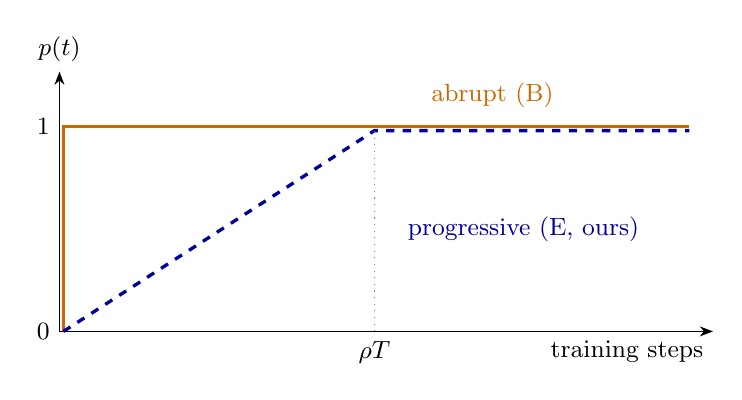
\begin{tikzpicture}[x=1cm,y=1cm]
  \draw[-{Stealth}] (0,0) -- (8.3,0) node[below left] {\small training steps};
  \draw[-{Stealth}] (0,0) -- (0,3.3) node[above] {\small $p(t)$};
  \node[left, font=\small] at (0,2.6) {1};
  \node[left, font=\small] at (0,0) {0};
  \draw[orange!80!black, very thick] (0.05,0) -- (0.05,2.6) -- (8,2.6);
  \draw[blue!60!black, very thick, dashed] (0.05,0) -- (4,2.55) -- (8,2.55);
  \draw[gray, dotted] (4,0) -- (4,2.55);
  \node[below, font=\small] at (4,0) {$\rho T$};
  \node[font=\small, orange!80!black, anchor=west] at (4.6,3.0) {abrupt (B)};
  \node[font=\small, blue!60!black, anchor=west] at (4.3,1.3) {progressive (E, ours)};
\end{tikzpicture}
\caption{Probability of encoding a training sequence with the new tokenizer.}
\label{fig:schedule}
\end{figure}

\paragraph{Why code and Chinese.} The two domains are deliberately far apart. Code is close to English: new code tokens (\texttt{return}, \texttt{self.}, \texttt{import}) split into English pieces that GPT-2 already knows, so FVT gives a good initialization and the abrupt swap should hurt little. Chinese is far from English: new Chinese tokens split into raw UTF-8 bytes whose GPT-2 embeddings carry little meaning, so FVT helps less and the abrupt swap should hurt more. For Chinese we first run a lighter version of the Phase~1 tokenizer grid on Chinese and English Wikipedia (data mix, GPT-4 regex versus Identity, 32k and 50k tokens).

\paragraph{Conditions.} On both code and Chinese we compare A (keep GPT-2 tokenizer), B (abrupt swap with FVT) and E (progressive swap with FVT, ours), at 50M and 200M tokens. On code, A and B are reused from Phase~1.

\subsection{Phase 3 (optional): cheaper inference}
With a fixed vocabulary, a text can usually be segmented with fewer tokens than greedy BPE merges produce, by choosing the segmentation with the minimum number of tokens (a shortest-path search). Standard models degrade on such unusual segmentations. Because model E is trained on two different segmentations, it may be more robust to them. If time allows, we will measure the trade-off between token count and bits per byte under shortest-path encoding for models B and E.

\subsection{Metrics and compute}
\begin{itemize}
  \item \textbf{Bits per byte} on held-out code or Chinese text (primary metric). Per-token perplexity is not comparable across tokenizers, so we normalize the total negative log-likelihood by the number of UTF-8 bytes:
  \begin{equation}
    \mathrm{bpb} = \frac{-\sum_t \log_2 p(x_t \mid x_{<t})}{\#\text{bytes}}.
  \end{equation}
  \item \textbf{Training-loss curves} in bits per byte, to observe the loss spike after an abrupt swap.
  \item \textbf{Generation speed} in characters per second, to measure the practical gain of the new tokenizer.
  \item \textbf{MBPP pass@$k$}~\citep{austin2021mbpp} on code, reported only if a 124M model scores clearly above zero.
\end{itemize}

\paragraph{Compute.} Training a 124M model costs about $6 \times 1.24\times10^{8}$ FLOPs per token. We measured the training throughput of GPT-2 small on the RTX 5050 of our cluster (bf16, sequences of 1{,}024 tokens, Table~\ref{tab:speed}). The output layer dominates memory: with the 80k-token union vocabulary of Phase~2, a micro-batch of 4 sequences no longer fits in 8\,GB. We therefore train with micro-batches of 2 and 32 accumulation steps (65{,}536 tokens per optimizer step). A 50M-token run takes about 1 hour and a 200M-token run 4 to 5 hours. The full plan (Phase~1: 6 runs; Phase~2: E on code plus A, B and E on Chinese, 8 runs) totals about 37 GPU-hours, which we will split across our three cluster accounts.

\begin{table}[h]
\centering
\caption{Measured training throughput of GPT-2 small on one RTX 5050 (8\,GB).}
\label{tab:speed}
\begin{tabular}{lrrrr}
\toprule
Vocabulary (conditions) & Micro-batch & Tokens/s & 200M tokens & Peak memory \\
\midrule
32k, new tokenizer (B, C) & 2 & 15{,}002 & 3.7\,h & 3.8\,GB \\
50k, GPT-2 (A) & 4 & 12{,}697 & 4.4\,h & 7.2\,GB \\
80k, union (E) & 2 & 11{,}880 & 4.7\,h & 5.4\,GB \\
\bottomrule
\end{tabular}
\end{table}

\paragraph{Risks and fallbacks.} If compute runs short, we drop the 200M-token run of condition C and Phase~3. If the model relies too long on old tokens, we use a shorter ramp. If GPT-2 small proves too weak, Pythia-160M~\citep{biderman2023pythia} is an alternative base model.

%=====================================================================
\section{Expected Results}
\label{sec:expected}

We state our expectations as hypotheses. The only numbers below come from \citet{dagan2024tokenizer}; none are from our own experiments yet.

\begin{description}[leftmargin=0.9cm,style=nextline]
  \item[H1] \textbf{The paper reproduces at small scale (Phase 1).} The compression ranking on code should match the paper: Identity compresses the most, GPT-4 slightly more than Punct, with diminishing returns as the vocabulary grows. At 32k, the paper reports code NSL (relative to Llama) of 0.81 for GPT-4, 0.86 for Punct and 0.69 for Identity. FVT (B) should clearly beat random initialization (C); at 1.5B, the paper finds that removing FVT costs 2.1 points of HumanEval Pass@1. Model B should approach the baseline A by 200M tokens.
  \item[H2] \textbf{No loss spike with the progressive swap (Phase 2).} The abrupt swap starts with much higher bits per byte than the baseline. We expect E to avoid this spike and to reach lower target bits per byte than B at the 50M-token budget.
  \item[H3] \textbf{The farther from English, the larger the gain.} We expect the advantage of E over B to be small on code and larger on Chinese, because FVT already initializes code tokens well but not Chinese ones.
  \item[H4] \textbf{Cheaper inference (Phase 3, optional).} Model E should lose less quality than B under shortest-path encoding, allowing even fewer tokens per text.
\end{description}
If the progressive transition does not help, this remains an informative negative result: it would suggest that the cost of a tokenizer swap at small scale comes from learning new embeddings rather than from the abruptness of the change.

\begin{figure}[h]
\centering
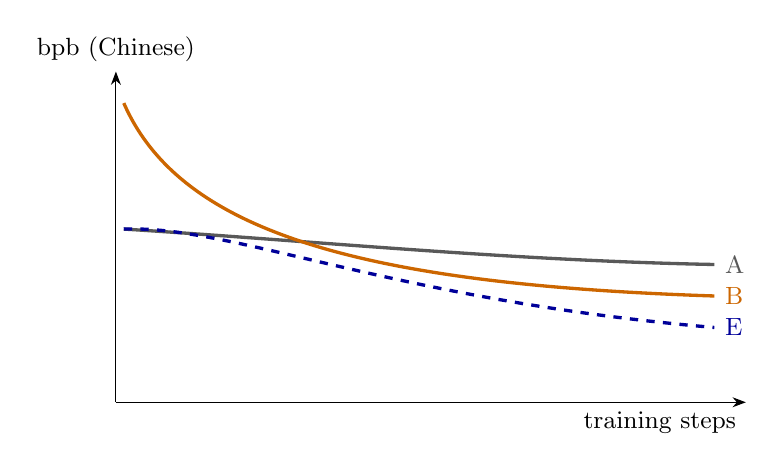
\begin{tikzpicture}[x=1cm,y=1cm]
  \draw[-{Stealth}] (0,0) -- (8,0) node[below left] {\small training steps};
  \draw[-{Stealth}] (0,0) -- (0,4.2) node[above] {\small bpb (Chinese)};
  \draw[gray!70!black, very thick] (0.1,2.2) .. controls (2.5,2.05) and (5,1.8) .. (7.6,1.75) node[right] {\small A};
  \draw[orange!80!black, very thick] (0.1,3.8) .. controls (0.8,2.2) and (3,1.5) .. (7.6,1.35) node[right] {\small B};
  \draw[blue!60!black, very thick, dashed] (0.1,2.2) .. controls (1.5,2.25) and (3.5,1.3) .. (7.6,0.95) node[right] {\small E};
\end{tikzpicture}
\caption{Hypothesis sketch for Chinese, not data. A: keep GPT-2 tokenizer; B: abrupt swap with FVT; E: progressive swap.}
\label{fig:sketch}
\end{figure}

\paragraph{Planned timeline.} Weeks 1--2: Phase~1 (code tokenizer grid, runs A--C). Weeks 3--5: Phase~2 (union vocabulary and mixed data loader, Chinese tokenizer grid, runs on code and Chinese). Week 6: Phase~3 if time allows, analysis and final report.

\bibliographystyle{plainnat}
\bibliography{references}

\end{document}
